\def \kaflanr {8}
\lecture[\kaflanr]{\kaflanr. Stiglar}{lecture-text}
\date{28.~janúar 2015}
\newcounter{mycount}
\refstepcounter{mycount}

\begin{document}

\subsection{}
	\maketitle





\subsection{Stigull} 

\subsubsection{Skilgreining \kaflanr.\arabic{mycount}}\stepcounter{mycount}

 Látum $f(x,y)$ vera fall og $(x,y)$ punkt þar
sem báðar fyrsta stigs hlutafleiður $f$ eru skilgreindar.  Skilgreinum
{\em stigul} $f$ í punktinum $(x,y)$ sem vigurinn 
$$\nabla f(x,y)=f_1(x,y)\iv+f_2(x,y)\jv.$$
Stigull $f$ er stundum táknaður með {\bf grad}$\,f$.








\subsection{Stigull} 

\subsubsection{Ritháttur \kaflanr.\arabic{mycount}}\stepcounter{mycount}
Oft hentugt að rita
$$\nabla=\iv\frac{\partial}{\partial x}+ \jv\frac{\partial}{\partial y}.$$
Þá er litið svo á að $\nabla$ sé {\em diffurvirki}, þ.e.a.s.\ $\nabla$
gefur fyrirmæli um hvað á að gera við $f$ til að fá $\nabla f(x,y)$.




\subsection{Dæmi}
 \begin{figure}[!h]
        \centering
        \begin{minipage}{.5\textwidth}
            \centering
            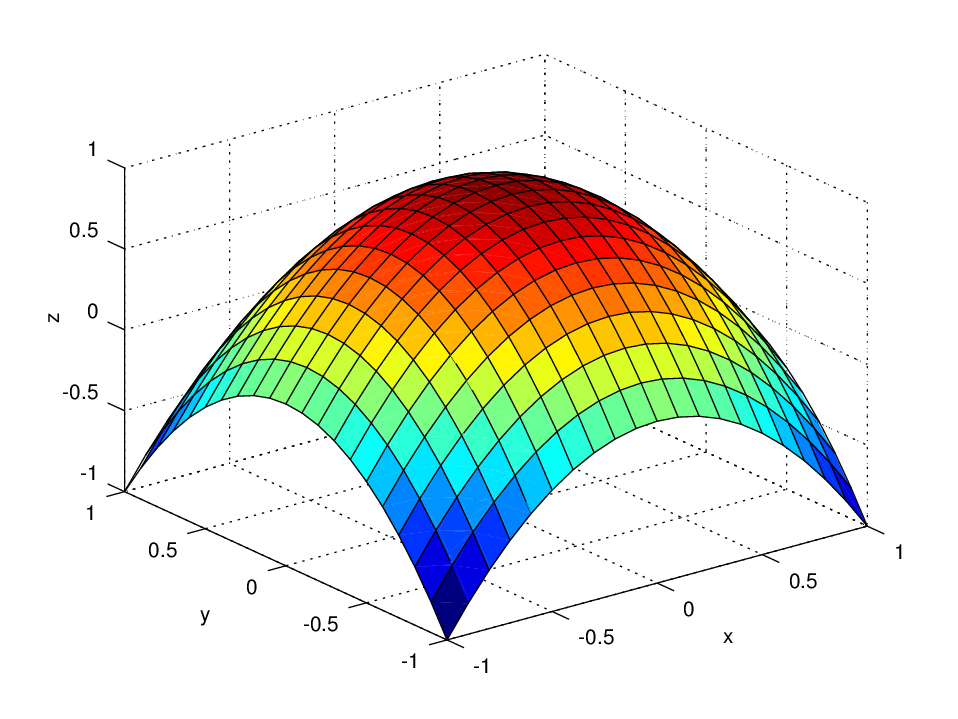
\includegraphics[width=1\linewidth]{gradfurf.png}
            \caption*{Graf $z=1-x^2-y^2$}
        \end{minipage}%
        \begin{minipage}{.5\textwidth}
            \centering
            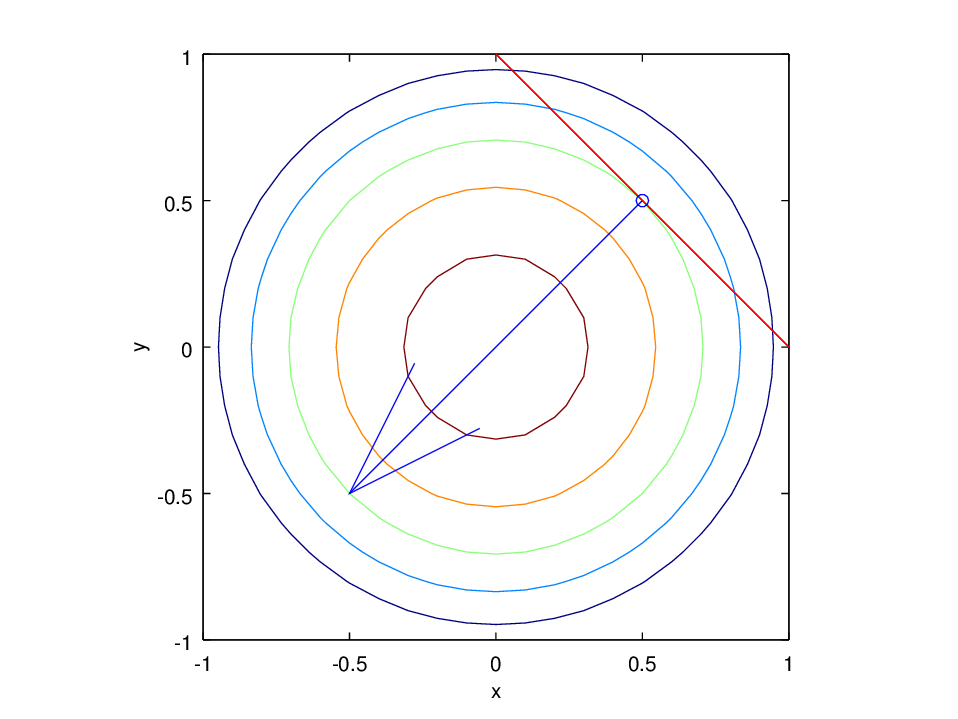
\includegraphics[width=1\linewidth]{gradient.png}
            \caption*{Jafnhæðarlínur.  Stigull og snertilína við jafnhæðarlínuna $z=0.5$ í $(x,y) = (0.5,0.5)$.}
        \end{minipage}
    \end{figure}
 




\subsection{Stigull} 

\subsubsection{Setning \kaflanr.\arabic{mycount}}\stepcounter{mycount}
  Gerum ráð fyrir að fallið $f(x,y)$ sé
diffranlegt í punktinum $(a,b)$ og að $\nabla f(a,b) \neq \mathbf{0}$.  Þá er vigurinn $\nabla f(a,b)$ 
hornréttur á þá jafnhæðarlínu $f$ sem liggur í gegnum punktinn $(a,b)$.
%Rissum sönnun. Þurfum að gefa okkur að hægt sé að stika jafnhæðarlínu með diffranlegum stikaferli.








\subsection{Snertilína við jafnhæðarferil} 

\subsubsection{Setning \kaflanr.\arabic{mycount}}\stepcounter{mycount}
  Gerum ráð fyrir að fallið $f(x,y)$ sé
diffranlegt í punktinum $(a,b)$ og að $\nabla f(a,b) \neq \mathbf{0}$.  Jafna snertilínu við jafnhæðarferil $f$ í punktinum $(a,b)$ er gefin
með formúlunni 
$$\nabla f(a,b)\cdot (x,y)=\nabla f(a,b)\cdot (a,b),$$
eða 
$$f_1(a,b)(x-a)+f_2(a,b)(y-b)=0.$$




\subsection{Stefnuafleiða} 

\subsubsection{Skilgreining \kaflanr.\arabic{mycount}}\stepcounter{mycount}
 Látum $\uv=u\iv+v\jv$ vera einingarvigur.  {\em
  Stefnuafleiða } $f$ í punktinum $(a,b)$ í stefnu $\uv$ er skilgreind
  sem 
$$D_{\uv}f(a,b)=\lim_{h\rightarrow 0^+}\frac{f(a+hu, b+hv)-f(a,b)}{h}$$
ef markgildið er skilgreint.  




\subsection{Stefnuafleiða} 

\subsubsection{Setning \kaflanr.\arabic{mycount}}\stepcounter{mycount}
Gerum ráð fyrir að fallið $f$ sé diffranlegt í
$(a,b)$ og $\uv=u\iv+v\jv$ sé einingarvigur.  Þá er stefnuafleiðan í
punktinum $(a,b)$ í stefnu $\uv$ skilgreind og gefin með formúlunni
$$D_{\uv}f(a,b)=\uv\cdot \nabla f(a,b).$$




\subsection{Stefnuafleiða} 

\subsubsection{Setning \kaflanr.\arabic{mycount}}\stepcounter{mycount}
 Látum $f$ vera gefið fall og gerum ráð fyrir að
$f$ sé diffranlegt í punktinum $(a,b)$.

\medskip
(a)  Hæsta gildið á stefnuafleiðunni $D_{\uv}f(a,b)$ fæst þegar $\uv$
er einingarvigur í stefnu $\nabla f(a,b)$, þ.e.a.s. $\uv=\frac{\nabla
  f(a,b)}{|\nabla f(a,b)|}$.  

\medskip
(b)  Lægsta gildið á stefnuafleiðunni $D_{\uv}f(a,b)$ fæst þegar $\uv$
er einingarvigur í stefnu $-\nabla f(a,b)$, þ.e.a.s. $\uv=-\frac{\nabla
  f(a,b)}{|\nabla f(a,b)|}$. 

\medskip
(c)  Ef $\cal C$ er sú hæðarlína $f$ sem liggur í gegnum $(a,b)$ og
$\uv$ er einingarsnertivigur við $\cal C$ í punktinum $(a,b)$ þá er
$D_{\uv}f(a,b)=0$.  






\subsection{Stefnuafleiða}
   \centering
            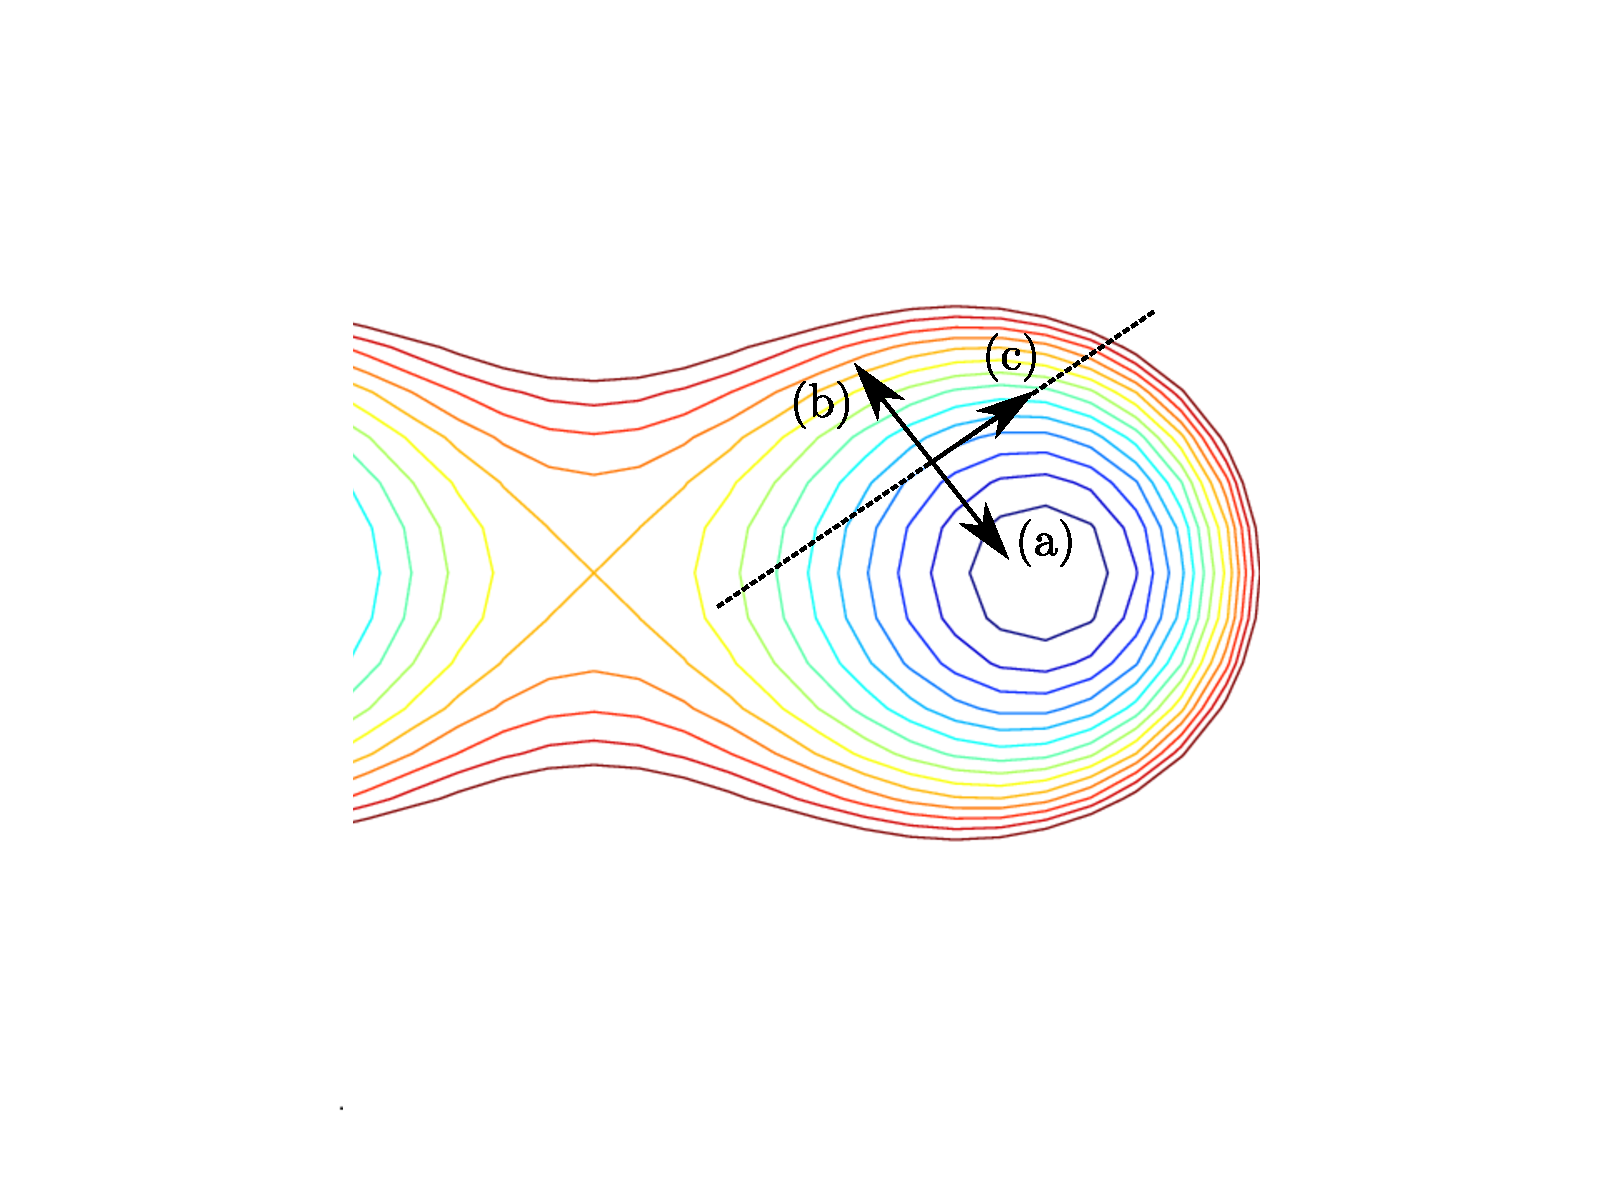
\includegraphics[width=1\linewidth]{contours.pdf}



\subsection{Stefnuafleiða} 

\subsubsection{Setning \kaflanr.\arabic{mycount}}\stepcounter{mycount}
Látum $f$ vera gefið fall og gerum ráð fyrir að
$f$ sé diffranlegt í punktinum $(a,b)$.  

\medskip
(a) Í punktinum $(a,b)$ þá vex $f$ hraðast ef haldið er í stefnu
$\nabla f(a,b)$.  

\medskip
(b) Í punktinum $(a,b)$ þá minnkar $f$ hraðast ef haldið er í stefnu
$-\nabla f(a,b)$.  

\medskip
(c)  Ef $\cal C$ er sú hæðarlína $f$ sem liggur í gegnum $(a,b)$ og
$\uv$ er einingarsnertivigur við $\cal C$ í punktinum $(a,b)$ þá er
er vaxtarhraði $f$ í stefnu $\uv$ jafn 0. 




\subsection{Stigull} 

\subsubsection{Skilgreining \kaflanr.\arabic{mycount}}\stepcounter{mycount}
 Látum $f$ vera fall af þremur
breytistærðum, þannig að allar þrjár fyrsta stigs hlutafleiður $f$ í
punktinum $(x,y,z)$ séu skilgreindar.  {\em Stigull} $f$ í punktinum
$(x,y,z)$ er skilgreindur sem vigurinn
$$\nabla f(x,y,z)=f_1(x,y,z)\iv+f_2(x,y,z)\jv+f_3(x,y,z)\kv.$$





\subsection{Snertiplan við jafnhæðarflöt} 

\subsubsection{Setning \kaflanr.\arabic{mycount}}\stepcounter{mycount}
 Látum $f$ vera fall af þremur
breytistærðum þannig að fallið $f$ er diffranlegt í punktinum $(a,b,c)$.  Látum $\cal F$ tákna þann jafnhæðarflöt $f$ sem liggur um $(a,b,c)$.  Stigullinn $\nabla f(a,b,c)$ er hornréttur á flötinn $\cal F$ í punktinum $(a,b,c)$ og snertiplan (ef $\nabla f(a,b,c)\neq\ov$) 
við jafnhæðarflötinn í punktinum $(a,b,c)$ er gefið með jöfnunni 
$$\nabla f(a,b,c)\cdot(x,y,z)=\nabla f(a,b,c)\cdot(a,b,c)$$
eða með umritun
$$f_1(a,b,c)(x-a)+f_2(a,b,c)(y-b)+f_3(a,b,c)(z-c)=0.$$






\end{document}